\documentclass[12pt,fleqn,a4paper]{article}

\usepackage{latexsym}
\usepackage{url}
\usepackage{xspace}
\usepackage{epsfig}
\usepackage{psfrag}
\usepackage{a4wide}
\usepackage{marvosym}
\usepackage{amsmath,amsfonts,amssymb,amsthm,latexsym}
\usepackage{graphics,graphicx,color,subfigure}
\usepackage{fancyhdr}
\usepackage[english]{babel}
\usepackage[latin1]{inputenc}
\usepackage{float}
% added this package solely because "our" title is way too long and it
% allows to add a line break in the title
%\usepackage[usestackEOL]{stackengine}

\textheight 680pt
\textwidth 460pt
\topmargin -40pt
\oddsidemargin 5pt
\evensidemargin 5pt
\parindent 0pt

\pagestyle{fancyplain} \setlength{\headheight}{16pt}
\renewcommand{\sectionmark}[1]{\markright{\thesection\ #1}}
\lhead[\fancyplain{}{\thepage}]
  {\fancyplain{}{\rightmark}}
\rhead[\fancyplain{}{\leftmark}]
  {\fancyplain{}{\thepage}}
\cfoot{}
\renewcommand{\thesection}{\arabic{section}}
\renewcommand{\thesubsection}{\arabic{section}.\arabic{subsection}}


\begin{document}
\begin{titlepage}%Institution
\vspace{2cm}
\centerline{
\large{Department of Computer Sciences}}
\vspace{0.2cm}
\centerline{\large{University of Salzburg}}%Title with one or two Lines(More if wanted)
%\hline
\vspace{2cm}

\centerline{\large{PS Natural Computation}}
\centerline{SS 13/14}
\vspace{1cm}

\centerline{\Large{Design and implementation of a robot task}}
%\centerline{\Large{\bf\Longstack{SIMMA\\Design and implementation of a robot task\\demonstration the effect of
%neuromodulators}} }%Type of the Document
\vspace{1cm}

\vspace{0.4cm}%Date
\centerline{\today}
\vspace{5cm}%Authors

%\hline
\vspace{0.2cm}
Project Members:\\
\centerline{Tobias Auinger, 1220321, auingerto@stud.sbg.ac.at}\\
\centerline{Christian M\"{u}ller, 1123410, mueller110@gmx.net}\\
\centerline{Andreas Pollhammer, 9520061, pollhammerand@stud.sbg.ac.at}\\
\centerline{Stefan Schwarz, 1220024, schwarzst@stud.sbg.ac.at}\\
\vspace {0.8cm}\\

Academic Supervisor: \\
\centerline{Helmut MAYER}
\centerline{helmut@cosy.sbg.ac.at}
\vspace{0.8cm}\\
Correspondence to: \\
\centerline{Universit\"{a}t Salzburg} \\
\centerline{Fachbereich Computerwissenschaften} \\
\centerline{Jakob--Haringer--Stra\ss e 2} \\
\centerline{A--5020 Salzburg} \\
\centerline{Austria}
\clearpage
\end{titlepage}



%%%
%Table of Content
% \setcounter{page}{1}
% \pagenumbering{Roman} %I,II,III... in the TOC
% \tableofcontents

\clearpage
\pagestyle{headings}
\pagenumbering{arabic}  %Better if TOC is variable (more than one page)
\setcounter{page}{1}
\pagenumbering{arabic}  %Better if TOC is variable (more than one page)
\setcounter{page}{1}

\tableofcontents
\newpage

\abstract
{The main goal of this project is designing a task that demonstrates that the usage of neuromodulators can influence the evolution of a neural network in a positive way. For implementation and simulation of the task we use SIMMA "a simulation framework mainly developed for the simulation of mobile autonomous robots and their behaviour".}

%%%
\section{Introduction}
Our team, consisting of four people, designed a task for neural networks, to demonstrate that the usage of neuromodulators can influence the evolution of a neural network in a positive way.
In order to get the desired input-output mapping our neural network must be trained.
For that purpose Simma uses evolutionary Algorithms, which are algorithms that try to implement the principles of darwinian evolution with the purpose of training an artificial neural network. An artificial neural network consists of a set of neurons and each neuron receives one or more inputs. The sum of inputs is then passed to the activation function and further to the another neuron, until an output neuron is activated.
%A neural network consists of so called neurons. Each neuron receives one or more Inputs. The %output of is calculated by taking the sum of inputs as an input for the so called activation %function.

\begin{figure}[h]
\centering
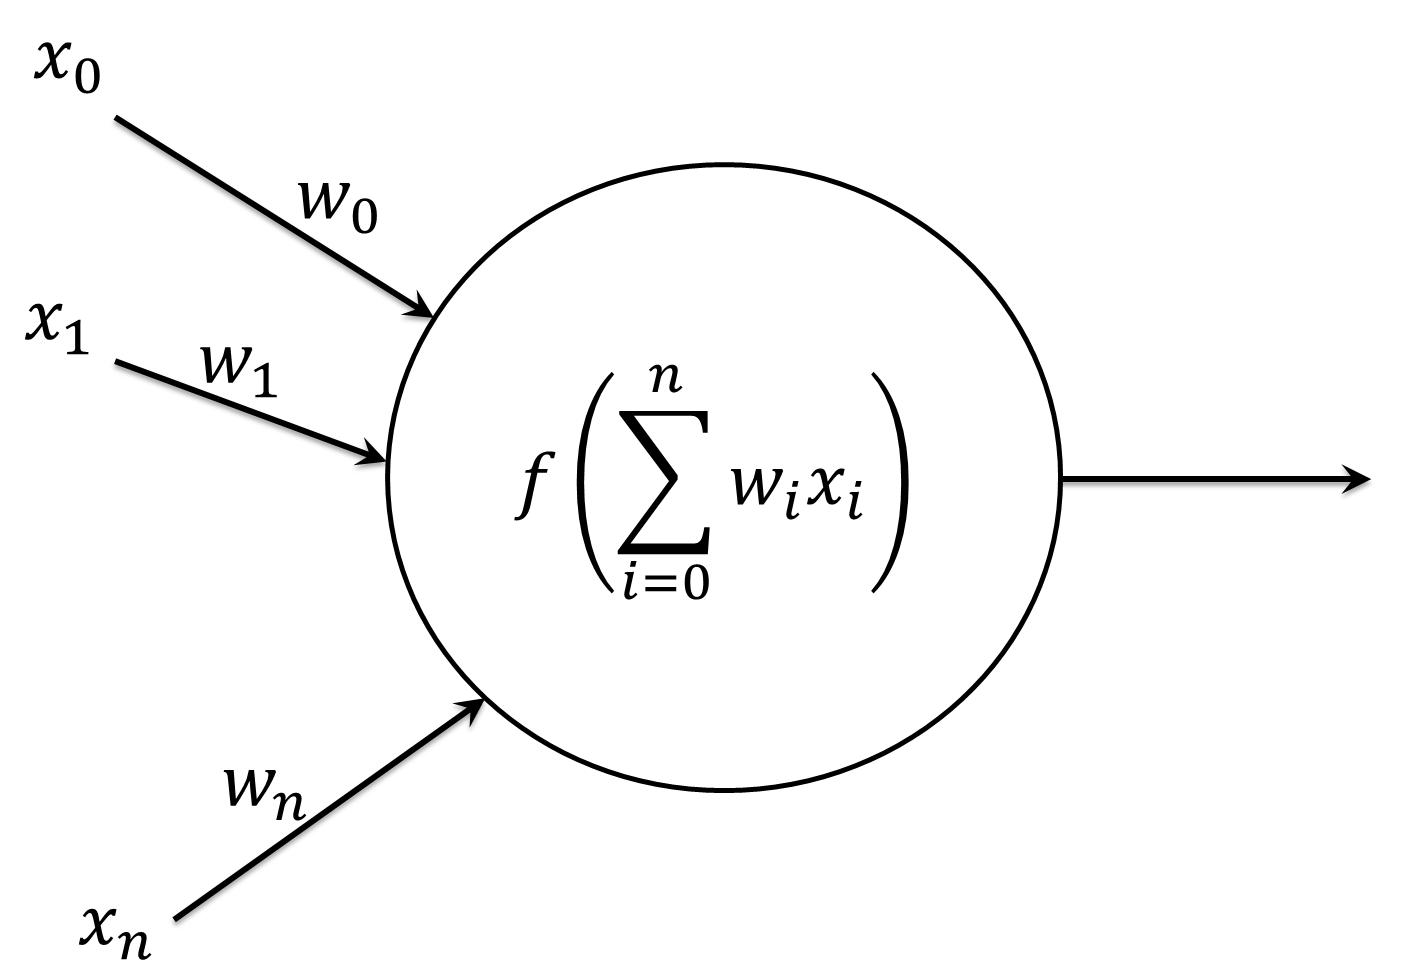
\includegraphics[scale=0.3]{img/neuron.png}
\caption{A neuron.}
\label{fig:neuron}
\end{figure}

In figure \ref{fig:neuron}

\subsection{SIMMA}

\section{Theoretical Foundation}
\subsection{Neuromodulation}
Neuromodulation basically describes a mechanism, which allows a neuron to switch between different states. There are different approaches how this may work in nature and also how neuromodulators are implemented in different variants of ANNs. In our case the mentioned states of the neuron are associated with a change of bias, the neurons output. In general, it is a complex problem, to find out in which cases bias changes would have a positive effect. So we simply left this to evolution.

For our project, we defined one neuromodulator using the SIMMA class\\ \texttt{simma.ann.modulator.BiasChange}. As Brain we selected the also already existing class \texttt{simma.ann.NeuroModulatorController}. See appendix for a complete listing (xml) of our setup.

\section{The Task}

\subsection{The initial task}
After careful considerations we decided to implement a robot whose task is to collect several pegs, which are randomly distributed within a virtual rectangular world and transport them to a certain place we call spot. While transporting the pegs to the spot the robot has to avoid collisions with one or more enemies following the robot. If the robot is captured by the enemy, it will get some damage, which effects its speed. The robot is supposed to learn this task by means of evolving neural networks. Our hope was that neuromodulators will indeed influence the evolution of our neural network in a positive way. So the neuromodulators assist our robot by learning this task. For implementation and simulation of the task we used SIMMA "a simulation framework mainly developed for the simulation of mobile autonomous robots and their behaviour". 

After several tests it turned out, that one part of the task worked very well. Namely the finding and collecting of the pegs, which includes the delivery to the spot. But to our disappointment robots trained to find and collect pegs, seemed to be unable to also learn how to avoid collisions with ghosts. So we focused on the second part of the task, the transportation of pegs through the enemy region.

\subsection{The final task}
For the final task, we divided the region of the simulation in three parts, each with a different purpose. The left side is where the spot spawns, which is the destination for the robots virtual delivery. The right side is the robot's
starting position. Right between those regions, the enemy, named ghost, spawns. This enemy's mere function is to stop the robot's delivery. The ghost does not move around randomly, but it detects the robot's current position for hunting it down, though it has been given a radius in which the robot is followed, which alters the size each new start, depending on the randomly generated number from 0 to 1. This so called "aggression potential" will also influence the robots fitness, given that the bigger this aggression potential is, the harder the robots mission will be. The virtual load carried by the robot does decrease its speed, making it easier to be targeted, since the robot does move slower (or at nearly the same speed, depending on the settings) with a full load than the ghost. Therefore the robot has to drop a certain amount of this load, in order to elude the ghost. By reaching the spot, hence fulfilling its task, the robot will drop the load, or what's left of it, and gains a specific amount of bonus. Does the robot fail its task, whether by getting caught, or not being capable of managing to deliver the load in the given time interval, then it won't have any fitness at all for this round of evaluation. If the ghost's aggression potential is too tiny, dropping a part of the load in order to increase the speed is not necessary, since the robot most likely won't be attacked, thus it should only deposit in need. 
The neuromodulators should simulate a panic reaction to the ghost's approach. This panic reaction should help the robot to recognize the right moment to drop a part of the load.
We used a smaller range of aggression potential for evolving the robot than for testing, hoping to see a better adaption of the neuromodulator based robots to this change.
Thence we thought seeing the effect of neuromodulators in the performing of this task

\subsection{The Fitness Function}
After putting a lot of thought in to the fitness function, we decided to evaluate with the following criteria:
\[ fitness = \frac{\sum_{i=0}^{episodecount} (bonus_i + load_i)*Aggressionpotential_i}{episodecount} \]
The main goal of the robot is to reach the spot with a maximum amount of pegs. 
If the robot did not manage to reach the spot, the fitness will be 0 for its current episode.
In contrast to our expectations, prior to the testing of our task, the amount of bonus the robot gets just for reaching the spot is of a fundamental importance. If it is too low or not existent the robot will not drop it's pegs. For the individual itself this behaviour may result in death, but the missing survival bonus does not influence the population's fitness significantly. If it is too high the robot drops too many pegs. Some may argue that the above statements are false, because of the nature of a bonus.
The survival bonus is, as its name implies, just a bonus the robot gets on top of its regular performance.

\subsubsection{Considerations on how to improve the robots performance}
When watching the robots movements, it sometimes seems that the robot fails to avoid a collision with the ghost, because there is not enough space within the rectangular world. This happens when the robot tries to gain distance from the ghost while driving against a wall (outer border of the simulated world). We concluded, that this could possibly hinder the robot within its learning process, since there is no way for the robot to even recognize the existence of a wall, besides the fact, that the distance to the ghost does not rise as is should. But the robot could not determine, whether if this is a wall-problem, or the ghost is just faster than the robot. In the former case it should turn around without the need of dropping any pegs. And in the other case it should do just the opposite and drop some pegs. So being aware of this problem, we added the damage-sensor, which we already implemented for our previous task and used it to subtract one damage-point every time the robot collides with the wall. Additionally we added the compass (an existing sensor class in SIMMA) to give the Robot some kind of orientation. By also taking regard of the damage value within the fitness-function, we had been looking forward to evolve a robot which is learning to keep a little distance from the borders of the simulated world. This worked very well as long as we made it easy for the robot to solve the task, meaning a slow moving ghost with only low aggression potential. But with a higher degree of difficulty of the robots task, we were not able to identify any significant improvements. It seemed that the additional sensors just added complexity to the learning process without increasing the level of the reachable fitness. So we returned to our initial keep-it-simple approach.


\section{Components}
To simulate our task we need an area limiting the space, a robot, the delivery destination and an enemy. The limited space is represented by a rectangular area 1.07 meters wide and 0.7 meters in height. The other three components are described in further sections.

\subsection{The Robot}
The circle-shaped robot powered by a battery is our protagonist, which will be evolved to fulfill a certain task. It is able to move around the simulation area using its two wheels.
%An important factor of the performance is the speed. It is influenced by the carried amount of %load, making a fully loaded robot slower and therefore easier to catch.

\begin{figure}[h]
\centering
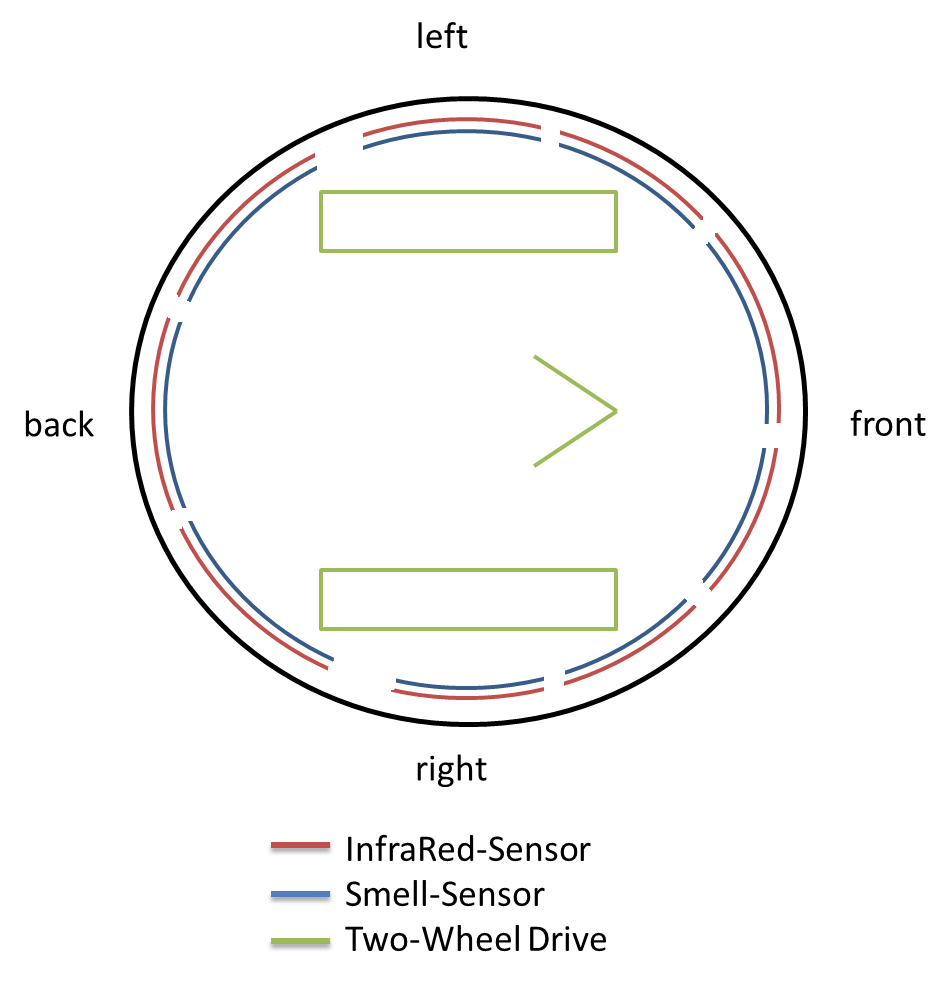
\includegraphics[scale=0.333]{img/robot_neu.png}
\caption{The robot with its sensors and wheels.}
\label{fig:robot}
\end{figure}

\subsubsection{Sensors}
The robot is equipped with the following sensors:
\begin{itemize}
   \item 1 Load-Sensor
   \item 9 Smell-Sensors
   \item 9 Infrared-Sensors
\end{itemize}
The carried load is managed by the load sensor. Nine "smell sensors", which are attached around the robot, give him the ability to see the spot by receiving its produced smell. Determining the distance to the ghost is done by receiving the ghost's emitted heat through nine infrared sensors placed around the robot.

\subsubsection{Damage}
After a collision has been detected between the ghost and the robot, the robot is harmed, the robot's capability of movement is declined and therefore the robot failed its task, resulting in a fitness of 0.

\subsubsection{Actuator}
We extended the already existing class "TwoWheelDrive" with a third neuron. Originally there were two neurons: one for the right wheel and one for the left wheel. Our third neuron is the "peg-dropper-neuron". If the value of the neuron is greater than 0.5 the robot drops a certain amount of pegs, which lightens the robot, causing it to speed up.

\subsection{The Enemy}

The Enemy, called ghost is represented in SIMMA by a white circle. We therefore implemented a class called \texttt{Ghost}, for which the following settings can be made in the configuration-file: The speed of the ghost can be set by a tag called \texttt{Speed} with properties \texttt{VX} and \texttt{VY} for the speed in direction of the x-axis or y-axis respectively. The settings for \texttt{MoveArea} were intended to capture the ghost within a given aria, but are not used at current. Its one and only purpose is to hunt down the robot, making him unable to fulfill the delivery.

\subsection{The Spot}
The spot, being the delivery destination, is emitting smell in every direction of the simulation space, making it recognizable and distinguishable from the ghost. It also serves the purpose as a safe zone for the robot.

\section{Results}
For the results we evolved two robots, distinguished by the usage of neuromodulators and therefore a different brain. Despite of that, everything had to be equivalent for the comparison of those robots.
\newpage

\subsection{Evolution}
The following diagram (figure \ref{fig:diagram1}) shows an example of the evolution progress, with and without neuromodulators. As aggression potential we took a random value from the range of 0.3 to 0.8 for each episode. It is impotant to mention that this graph is not representative as it is just the product of a single evolution run.
\begin{figure}[h]
\centering
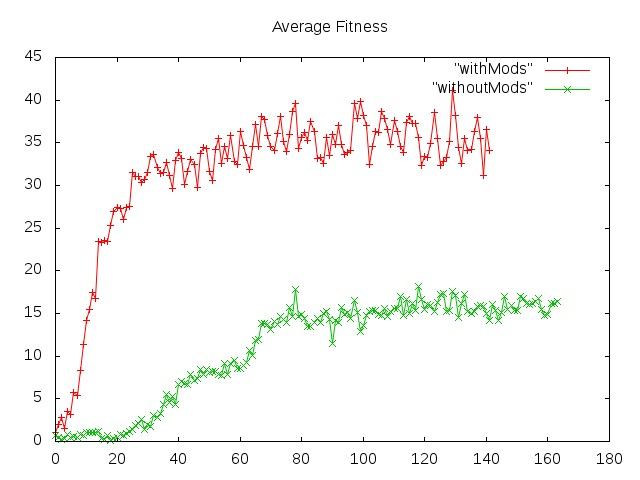
\includegraphics[scale=0.7]{img/evoAvg.jpg}
\caption{evo}
\label{fig:diagram1}
\end{figure}

The x-axis shows the number of generations and the y-axis represents the fitness reached.

\subsection{Performance}
We tested two of our evolved robots. The following diagrams compare the performance of the robot without neuromodulators (1) with neuromodulators (2). Diagram diagram (figure \ref{fig:diagram2}) shows the distance between the robot and the ghost, when the robot is dopping pegs. The robot should drot pegs only as a last resort, when it is attaced by the ghost. So we assume, that this distance as a good indicator of the robots performance.

\begin{figure}[H]
\centering
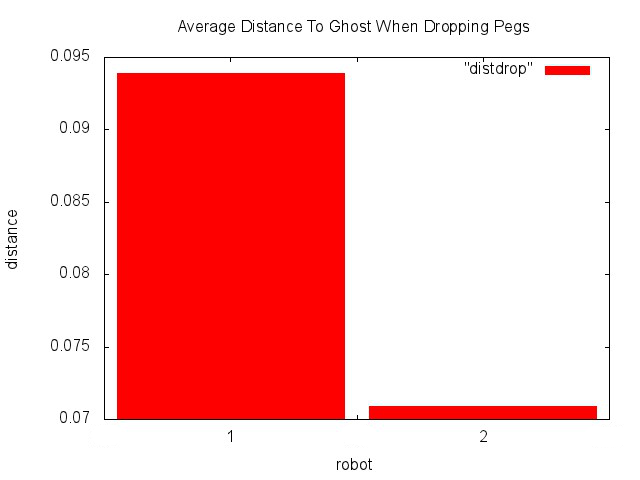
\includegraphics[scale=0.5]{img/distdrop_plot.png}
\caption{Average Distance}
\label{fig:diagram2}
\end{figure}

The secon diagram \ref{fig:diagram3}) shows the total count of drpped pegs on the way to the spot. Our robot without neuromodulators drops 100\% of all pegs, the other one only view.

\begin{figure}[H]
\centering
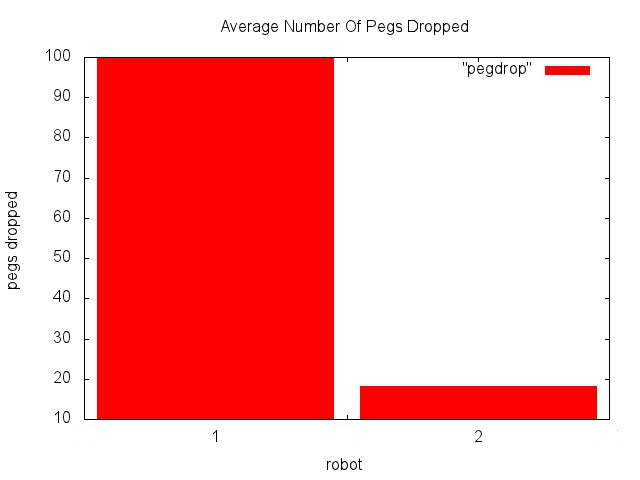
\includegraphics[scale=0.5]{img/pegdrop_plot.png}
\caption{Pegs dropped}
\label{fig:diagram3}
\end{figure}


\begin{figure}[H]
\centering
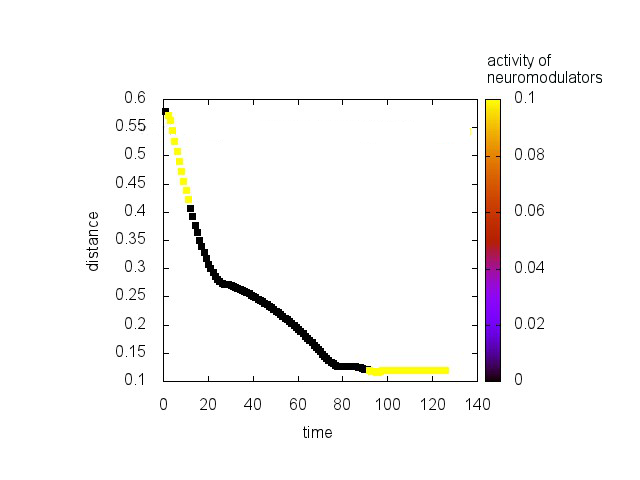
\includegraphics[scale=0.5]{img/dose_plot.png}
\caption{Activation of neuromodulators}
\label{fig:diagram4}
\end{figure}


\newpage

\section{Conclusion}
%By evolving and comparing those two robots with our implemented task, we noticed a positive %influence not only in performance, but also in the evolution, as we hoped to achieve.
It's difficult to find a clear statement about the differences between the evolution of a robot with or without the use of neuromodulators. Although we have seen a clear advantage for networks with neuromodulators in most cases, we have also seen some result indicating the opposite. But bringing all together, our conclusion is, that it is very suggestive to assume, that neuromodulators on the one hand cause a slower evolution progress, but on the other hand increase the reachable level of fitness. These findings are strongly connected to the task we have implemented. Future research in this field will probably show a more common applicability of these characteristics.

\section{Problems}
The old signal function:
\[signal += \frac{quantum}{(1 + \exp(0.65 * (dist - so.getBoundingRadius()) - (14.0 * \cos(1.3 * \alpha))))}\]
Our new signal function:
\[signal += \frac{quantum}{(1 + \exp(3.0 * (dist - so.getBoundingRadius()) - (2.5 * \cos(1.3 * \alpha))))}\]

\newpage
% links go here, NOT in references
%%%
\section{Links}

\begin{itemize}
\item Project Page: \url{http://student.cosy.sbg.ac.at/~cmueller/natcomp/}
\item PS Page: \url{http://www.cosy.sbg.ac.at/~helmut/Teaching/NaturalComputation/proseminar.html}
\end{itemize}

%\bibliography{}  % .bib files here

\begin{thebibliography}{1}
\bibitem{haykin}Simon Haykin {\em Neural Networks and Learning Machines} 2009: Pearson Education, Inc..
\bibitem{thesis}Esther Lo {\em Master Thesis: Neuromodulation in Artificial Systems} 2012: University of Oklahoma.
\end{thebibliography}


\end{document}


